\chapter{本科毕业论文外文翻译}
%字数要求3000字

\heiti
标题

\songti
Networking Named Content 内容命名网络

\heiti
作者

\songti
Van Jacobson, Diana K. Smetters, James D. Thornton, Michael F. Plass, Nicholas H. Briggs,
Rebecca L. Braynard

\heiti
机构

\songti
Palo Alto Research Center Palo Alto, CA, USA

\heiti
通讯方式

\songti
\{van,smetters,jthornton,plass,briggs,rbraynar\}@parc.com

\heiti
摘要

\songti
当今世界,网络已被内容(content)的传播和获取所主导,而网络技术却仍然只言主机间连接而不及其它。%其它指物,其他指人。
为获取网络内容和服务,须要建立起一个从网络用户所关心的(内容)到网络中的位置的映射。%需要主观且物质,须要客观且抽象
我们提出内容为心网络(Content-Centric Networking~简称~CCN)。它以内容为原语——把网络位置与网络身份、安全和访问分离开来,用名字访问内容。我们从IP推演出适用于命名内容的路由算法。使用这些算法,我们可以使网络的可扩展性、安全性和性能同时达到要求。我们实现了我们的体系结构的基本框架,用安全文件下载和VoIP电话两个例子演示了网络的性能和可恢复性。

\heiti
类别和学科描述符

\songti
C.2.1~[计算机系统组织]:网络结构与设计;~C.2.2~[计算机系统组织]:网络协议

\heiti
通用术语

\songti
设计,实验,性能,安全



%===========================%
\section{引言}
今天的互联网背后的工程原理和体系结构创建于二十世纪六、七十年代。网络致力于解决的问题是资源
共享的问题——远程使用如读卡器、高速磁带机甚至超级计算机等珍贵资源。这样产生的通信模型是一个仅仅存在于两台机器之间的对话模型,一台机器希望使用资源,另一台机器为前者提供资源。因此IP包含有两个地址,一个是发送方的,一个是目的地机器的,并且互联网上几乎所有的通信都包含TCP对话。

自包交换网络被创造的50年来,计算机及其附件已经成为廉价、普适的商品。互联网的连通性和低价的存储成本使得对海量新内容的访问成为可能——仅2008年就有500艾字节的信息被生产出来~[13]。人们在意的是互联网所承载的东西,而通信仍然在谈论这些东西都在哪些地方。

我们看到这个矛盾给用户带来三方面的(负面)影响。

\begin{description}
\item[可用性]为快速、可靠地访问内容,不仅须要如~CDN~和~P2P~网络这样繁冗的,预先设计好的,面向应用软件的机制,而且还会大幅增加带宽成本。
\item[安全性]对内容的信任这一概念被偷换为不那么可信的对物理位置和网络连接的的信任。
\item[位置迁就]建立从内容到物理位置的映射使网络服务的配置和实现工作都变得复杂。
\end{description}

解决这些问题的直接办法就是把网络中的“在哪里”(where)替换为“是什么”(what)。主机到主机对话是为了解决六十年代的问题而提出的抽象模型。对于如今的通信问题,我们认为命名数据(named data)是比命名主机(named hosts)更好的模型。我们提出内容为心网络(CCN),一个建立于命名数据之上的网络架构。即使是在CCN的最底层,我们也没有位置的概念——一个CCN包的“地址”是一个内容的名字,而不是这个内容的位置。不过,我们也保留了当年使~TCP/IP~简单、稳健、可扩展的那些设计决策。

\begin{figure}[htbp]
  \centering
  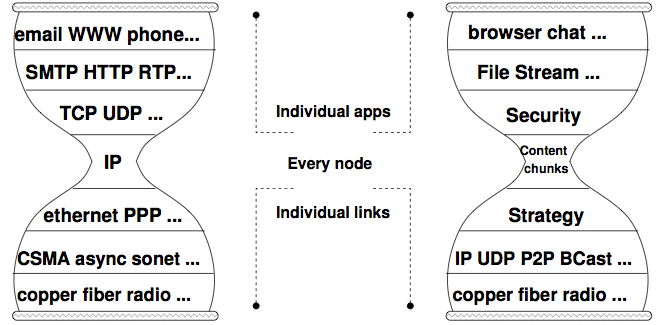
\includegraphics[width=0.7\textwidth]{images/narrow_waist}
  \caption{CCN~把网络协议栈中全局性的成分由IP换为了命名内容块} %不确定
  \label{narrow_waist}
\end{figure}

图~\ref{narrow_waist}~比较了~IP~和~CCN~协议栈。其中很多层都反映了双端约定;例如,第二层的成帧协议就反映了物理层上两端的约定,而第四层的传输协议就是一些信息生产者和消费者之间的约定。唯一一个需要全局约定的层就是第三层,即网络层。~IP~的成功在很大程度上要归功于它的网络层的简洁和它在网络第二层处提出的低要求,即:无状态,不可靠,无序,尽力交付。~CCN~的网络层(详见~\ref{sec:3})与~IP~的网络层很相似且~CCN~对第二层的要求更少,这使得它非常具有吸引力。除此之外,~CCN~可以单独成层,放置于任何一层之上,包括放置于~IP~层之上。%这一段我不是很清楚,尤其是最后一句

CCN~与~IP~有几点关键性的不同。其中两点即策略和安全已经以新层的方式在协议栈中展示了出来。由于~CCN~与第二层的关系更为简单,它可以最大限度地利用众多同时存在的网络的连通性(如以太网,~3G~,蓝牙和~802.11~等等)。~CCN~的策略层(详见~\ref{sec:3.3})为在不断变化的环境下最好地开发利用多种网络的连通性不断地做出细粒度、动态优化的选择。~CCN~确保的是内容本身的安全(详见~\ref{sec:5}),而不是内容走过的连接的安全。因此~CCN~没有许多基于主机网络的弱点,而不像~IP~网络那样深受其害。

我们在~\ref{sec:2}~至~\ref{sec:5}~中叙述了~CCN~的体系结构和运行方式。在~\ref{sec:6}~中我们评估了我们样板网络的性能。最后,在~\ref{sec:7}~和~\ref{sec:8}~中,我们讨论了相关工作并做出了结论。



%===========================%
\section{CCN~节点模型}
\label{sec:2}

\begin{figure}[htbp]
  \centering
  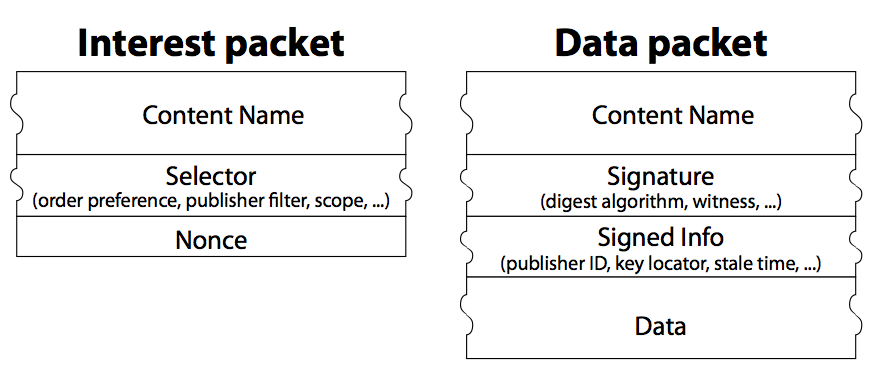
\includegraphics[width=0.7\textwidth]{images/packet_types}
  \caption{CCN~包的类型} 
  \label{packet_types}
\end{figure}

CCN~通信是由数据消费者驱动的。~CCN~包分为两类:兴趣包(Interest)和数据包(Data)(如图~\ref{packet_types})。消费者通过向所有连通之处广播自己的兴趣包来索要内容。任何一个收到兴趣包并且拥有满足该兴趣包的数据的节点都可以用一个数据包来回应该兴趣包。数据包仅为回应一个兴趣包而生,并且数据包产生之后这个收到的兴趣包就被“消费”了。
\renewcommand\baselinestretch{1} %调一下脚注行间距
\footnote{数据包和兴趣包因此是一对一的。它们保持这严格的流平衡。~TCP~中有一个类似的流平衡,即数据包和~ack~包之间的平衡。这一平衡赋予了~TCP~可扩展性和强适应性~[20]。然而与~TCP~不同的是,~CCN~模型对于多对多多点递送同样奏效(详见~\ref{sec:3.1})。}
因为兴趣包和数据包都用名字(name)来辨识内容,所以对同一个内容感兴趣的多个节点可以共享一个广播介质。其间只要使用标准的多播风暴抑制技术即可控制网络负荷~[3]。%不确定

如果兴趣包中的内容名字(ContentName)是数据包中内容名字的前缀,那么我们称数据包“满足”了兴趣包。~CCN~名字是由若干(显式确定数量的)名字部件(component)组成的不透明二元对象(如图~\ref{name})。名字一般是结构化的,因此如果前缀匹配则意味着数据包的名字是兴趣包的名字的子树(详见~\ref{sec:3.2})。~IP~使用了这种习惯来解析 <网络,子网,主机>这一层次结构。经验表明这样做既可以有效地将路由和转发状态结构化地集成,又可以支持快速查找。%极不确定
\renewcommand\baselinestretch{1} %调一下脚注行间距
\footnote{虽然~CCN~的名字是不定长的并且通常比~IP~地址要长,但是它们可以被高效地检索。一个~IP~地址的结构不是显式的,而是隐式地由节点的转发表决定的。因此,对~IP~查找使用现代~O(1)~哈希技术是十分困难的。所以~IP~查找通常使用~log(n)~的基数树检索或者并行但昂贵的~TCAMs~高端硬件。由于~CCN~的名字结构是显示的,内容名字可以很容易地被哈希,以便查找。}
这中匹配方式暗藏着这样一种可能性:内容尚未被生产出来,兴趣包就已经收到了——这使得发布者可以根据收到的数据请求实时地生产内容以回应兴趣。今天的网络中既有很多静态缓存着的数据,又有很多动态生成的数据,~CCN~灵活变化的名字机制使得它不论应对哪种数据都游刃有余。~CCN~名字还可以是上下文相关的,比如用~/ThisRoom/projector~与当前房间的投影仪交换信息,又如用~/Local/Friends~与本地(广播)环境上的任一好友交流。
\renewcommand\baselinestretch{1} %调一下脚注行间距
\footnote{这第二个例子会用到~CCN~签名机制产生的身份信息使好友们能用固定的名字约会而不是使用复杂的枚举或是探测算法。换言之,名字表示谈话的内容,而签名表示谈话者在上下文中的身份,如“本地的一个好友”。}

\begin{figure}[htbp]
  \centering
  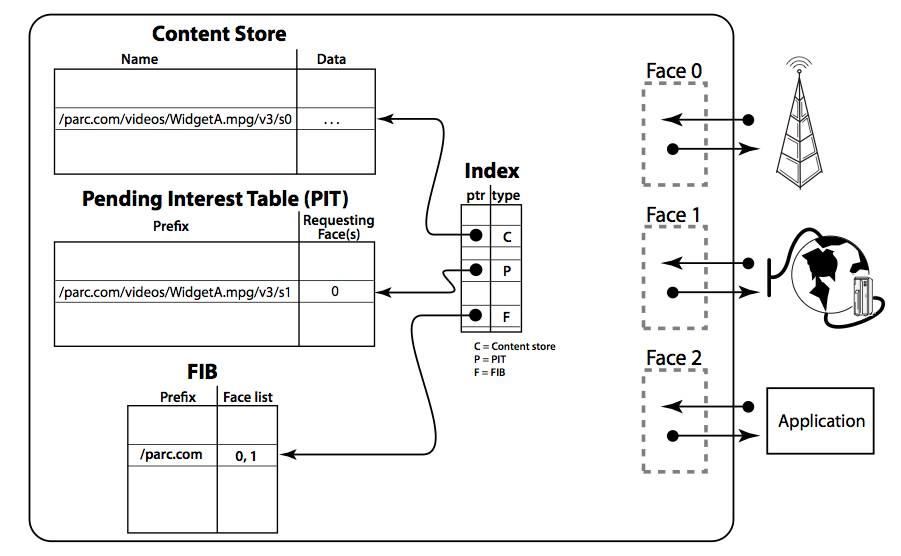
\includegraphics[width=0.7\textwidth]{images/engine}
  \caption{CCN~转发引擎模型} 
  \label{engine}
\end{figure}

CCN~节点的基本运营方式与~IP~节点非常相似:当一个包到达一个~face~时,(节点)会先做一个最长名字匹配,后续操作由匹配结果而定。
\renewcommand\baselinestretch{1} %调一下脚注行间距
\footnote{这里原文中使用了英文单词~face~而非~interface,因为包不仅仅是在硬件接口之间被转发,也被路由器内的应用程序处理(详见~\ref{sec:6})。}
图~\ref{engine}~展示了~CCN~的转发引擎。它有三个主要的数据结构:~FIB(Forwarding Information Base,转发中心),CS(Content Store,内容缓存)和~PIT(Pending Interest Table,待理兴趣表)。

FIB~用于将兴趣包转发给潜在数据源。它与~IP FIB~几乎相同,只是~CCN~的FIB会为每个兴趣包维护一个出口的列表,而~IP~的~FIB~仅需要为每个收到的包维护一个转发方向。这也反映了~CCN~在转发这方面并无限制这一事实。它允许多个数据源的存在,并允许并发地请求数据。

CS~与~IP~路由器的缓存大同小异,不过它们的置换策略略有不同。由于每个~IP~包仅仅属于一个点到点对话,它被转发了以后就不再具有任何意义了。因此~IP~路由器的做法是直接抛弃已转发的包并立即循环使用自己的缓存(MRU置换)。~CCN~包是幂等的,能够自我鉴别和自我认证,因此每一个~CCN~包都有被很多用户重用的潜力(如许多主机阅读同一份电子报纸或许多用户观看同一段~Youtube~视频)。为了使多个用户分享同一内容的概率最大化(这会带来上行带宽需求最小化和下行延时最小化等诸多裨益),~CCN~会尽可能多地储存到来的数据包(LRU或LFU置换)。

PIT~记录了数据包向数据源的转发记录,这样当数据包回到路由器时就可以按照~PIT~中的记录被转回至数据申请者(们)。在~CCN~中,只有数据包会被路由,并在它们走向潜在数据源的路上沿途撒下“面包屑”,以便匹配的数据将来沿着这些面包屑逆行,直到找到数据申请者(们)。每一个~PIT~表项就是这样一片面包屑。当一个~PIT~表项被用于转发数据包一次之后(即数据包“消费”了对应兴趣包),这个~PIT~表项就应该被抹去了。也有一些~PIT~表项一直都等不到匹配的数据包返回,这些表项最终必须因超时而被抹去(这时数据消费者如果仍然坚持想要那份数据,就有责任对那份数据重新表达兴趣)。

当兴趣包到达一个~face~时,一个最长名字匹配操作会被执行。匹配操作所用的索引结构(index)决定了机器会先在~CS~中寻找是否有匹配项,若没有则在~PIT~中寻找,若还没有则在~FIB中寻找。

如此,若本机的~CS~中已经有匹配兴趣包的数据包,则此数据包会从兴趣包到来的那个~face~被送出,然后兴趣包会被丢弃(因为它已经被满足了)。

如若不然,假如本机有一个~PIT~表项与兴趣包的内容名字完全匹配,则兴趣包到来的那个~face~会被加入到匹配的~PIT~表项中,然后那个兴趣包会被丢弃(因为这种情况表明对于相关数据的兴趣已经从本机向上行表达过了,现在需要确保的就是当对应数据包回到本机时必须向有新兴趣包到来的这个~face~抄送一份)。

若~PIT~中表项无一匹配,但是本机~FIB~中有匹配表项,那么这个兴趣包就必须根据匹配表项被转发。首先,在~FIB~对应表项的~face~列表中去除兴趣包到来的那个~face,若去除之后列表不为空的话,则将兴趣包转发给列表中的每一个~face。同时,一个新的~PIT~表项要被建立起来,这个表项的索引值是名字,内容是前面所说的~face~列表。

如果在~FIB~中都找不到与兴趣包匹配的表项,那么这个兴趣包会被直接丢弃(因为发生这种情况说明本机既没有现成的匹配数据,也不知道应该向哪里转发去寻找这个数据)。

相对于兴趣包而言,数据包的处理就要简单许多了。数据包不会被路由,它们只是简单地遵从沿路~PIT~表项的指示回到数据申请者(们)身边。当一个数据包到达时,也要做一次最长名字匹配。如果~CS~中有名字匹配则说明在此之前已经有数据包来过,所以这一个数据包就可以被丢弃了。如果有~PIT~匹配(可能不止一项),意味着此节点曾接收过对此数据包的请求。这个数据包可能先被验明正身(详见~\ref{sec:5.1})然后被加入~CS~(即~index~列表中指向该数据包的指针被标记为~C-type)。随后,将所有匹配的~PIT~表项中的请求~face~做集合并,再减去数据包的到达~face,对所得集合中的每一个~face,发出这个数据包。如果存在~FIB~匹配,则意味着~PIT~中没有匹配,或者说此节点从未收到过关于此数据包的兴趣但是数据包确来到了此节点。这个数据包是一个“不请自来”的数据包,应当被丢弃。
\renewcommand\baselinestretch{1} %调一下脚注行间距
\footnote{“不请自来”的数据包可能由恶意行为产生,也可能是有多个数据源,或者单一数据源但有多条数据传播路径。如果是后两种情况,第一个到达节点的数据包会把兴趣包消费掉,因此后来的数据包将会找不到相应的~PIT~表项。不论是何种情况,为了保证流平衡以及帮助维持网络的平稳运行,“不请自来”的数据包都应当被丢弃。}

节点的内存要用于多路复用,~CCN CS~模型允许将内存同时当做网络缓存使用,这点与~IP~的~FIFP~缓存模型不同。这样一来,所有的节点都可以提供缓存,缓存的大小仅仅受节点本身资源丰匮程度和管理政策的限制。

用兴趣包换取数据包这种方法使~CCN~本能地适用于多点通信,这使它在高度动态变化的环境中仍然能轻松维持通信。任何一个对多个网络持有访问权的节点都可以成为网络间的内容路由。一个移动节点通过使用自身缓存可以连通两个原本不相连的网络区域,或通过间歇连接提供延时连通性。~CCN~以此提供对容断网络(Disruption Tolerant Networking)~[11]~的支持。兴趣包和数据包的交换在有本地连通性的地方即可进行。例如,两个同事可以用他们的笔记本电脑和自组无线网络在一个与外界网络隔绝的地方正常地分享文件等等。

%===========================%
\section{传输}
\label{sec:3}
CCN~传输被设计为在不可靠包递送服务之上运行,包括在连通性高度变化的移动和普适计算设备中运行。因此兴趣包和数据包都可能在传输中被丢失或损坏,被请求的数据也有可能暂时无法访问。为了提供可靠的传输服务,在合理时间内未被满足的~CCN~兴趣包必须重传。与~TCP~不同,~CCN~的发送者是无状态(stateless)的。在已表达的兴趣无响应的情况下,如果对相关数据仍有兴趣,那么数据的最终消费者(即对数据感兴趣的那个应用程序)应当负责重新表达兴趣。数据接收方的~strategy layer~(详见图~\ref{narrow_waist})负责重传,同时负责决定用于表达兴趣的通信接口数、同一时间未被满足兴趣的最大容许量、不同兴趣之间的相对优先级等等。%存疑

底层的包交换网络可能会使包重复;~CCN~的多点传播模式(multipoint distribution)也可能造成包重复。根据~\ref{sec:2}~所述的节点运营机制,所有重复的包都会被丢弃。至此,虽然数据包的传播不会成环,但是兴趣包的传播却可能成环。这样,就有可能存在有的~face~收到了兴趣包,而实际上这个兴趣已经不存在了(被满足了)这样的局面。为了检测和预防此类事件,兴趣包中包含了一个随机数(nonce)。这样,从不同路径收到的重复的兴趣包就可以被丢弃了(见图~\ref{packet_types})。

CCN~兴趣包使用~TCP ack~包使用的流控制和定序方法。%function 不知道我译得对不对
流控制在~\ref{sec:3.1}~中详述。定序在~\ref{sec:3.2}~中陈述。由于节点能见到与它的兴趣包匹配的所有数据这一点是有保障的,对兴趣包的回应时间和回应率可以由节点直接测量并用于决定对于某些名字前缀的兴趣包应该采取何种策略。这些内容将在~\ref{sec:3.3}~中详陈。

%...............................................................%
\subsection{可靠性与流控制}
\label{sec:3.1}
一个兴趣包最多能带回一个数据包。这一基本规则保证了网络中的流平衡,使位于速度迥异的两个网络上的机器也能有效沟通。不过,与~TCP~中一样,可以将数据和请求合并。如果有多个兴趣包要发送,也不必等到第一个数据包回来消费了第一个兴趣包以后才发出第二个兴趣包,而是可以将多个兴趣包一起发出。兴趣包相当于~TCP~的窗口通告(window advertisement)。接收方可以通过调整它发出的兴趣包的数量来动态调整自己的窗口大小。我们在~\ref{sec:6.2}~中展示了这种流水化的效果。由于每一个~CCN~包都是独立命名的,这条流水线不会因为有的包丢失了而堵塞——~TCP SACK~技术所做的事情是~CCN~的本能之一。

在大型网络中,~TCP~对话端对端的本性决定了一个事实:即使每一个对话都保持着流平衡,发送方和接收方之间还是有很多地方会因为会话的汇聚(aggregation)而发生拥塞(congestion)。%拥塞的产生原因有三种:speed mismatch, aggregation, confluence
这种拥塞的后果是包的延时和丢失。对此,~TCP~的解决办法是让端点动态调整窗口大小,使汇聚流量低于发生拥塞的标准~[20]。之所以需要这样的流控制方法,其根本原因就在于~TCP~的流平衡是端对端的。在~CCN~中,所有通信都是基于本地的,所以发送方和接收方之间没有一点是不处于平衡状态上的。由于~CCN~的每一跳都在维持流平衡,就没有必要再用其它的技术去控制传输路径中的拥塞了。这与逐跳流控制(hop-by-hop flow control)是不同的。逐跳流控制使用相邻节点间背压(backpressure)来调整连续流的速率;~CCN~则没有~FIFO~队列,只有~LRU~缓存。这一设计可以拆解逐跳反馈形成的环,也可以一只振荡。(我们将在未来的一篇论文中详细讨论这个问题)

	
%...............................................................%	
\subsection{定序}
\label{sec:3.2}
在一个~TCP~对话中,数据的辨识要依靠序列号。相比序列号而言,~CCN~需要一些更复杂的东西:~CCN~的消费者们要从海量的数据之中申请一份,并且众多的消费者还可能分享同样的数据。~CCN~对数据的定位和分享依靠的是结构化的、聚合而成的名字。这些名字并不仅仅是一场转瞬即逝的对话中使用到的临时序列号。组成这些名字的至少部分部件是人们可读、可理解的,并且反应了数据的来历信息。虽说~CCN~的名字拥有这些内涵,当它们出现在兴趣包里的时候,它们的通信功能跟~TCP ACK~的功能是一模一样的:道明接受者需要的下一个数据。

\begin{figure}[htbp]
  \centering
  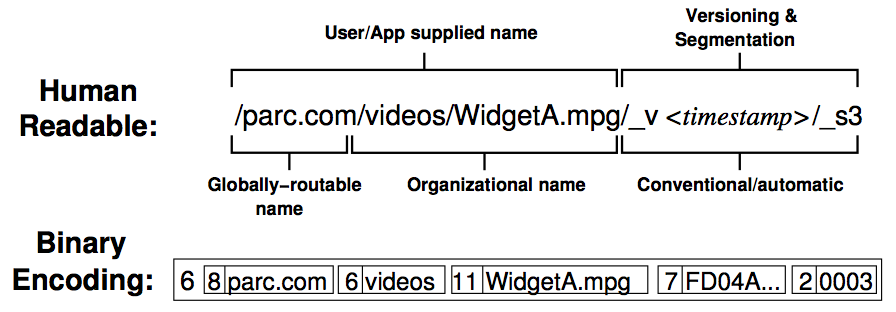
\includegraphics[width=0.7\textwidth]{images/name}
  \caption{名字示例} 
  \label{name}
\end{figure}

在我们细说数据的辨识机制以前,让我们先来谈谈~CCN~的名字。如前文所说,名字是结构化的;每一个名字都由若干个名字部件(component)组成。每个名字部件又是由若干个八位字节任意数组成的。在此,八位字节任意数是一种对~CCN~通信无影响的变长二进制数。名字必须对协议栈中的高层有意义,但是传输本身不对名字加任何额外的限制,只是要求名字必须结构化,必须由部件组成就够了。整数或其它复杂数值的二进制编码可以直接做名字部件使用,无须专为传输需要转化为文本。名字部件甚至可以出于安全需要而被加密。为了表示方便,我们用类似~URI~的格式书写名字,并用~\slash~分隔各个名字部件(如图~\ref{name}),但是这些分隔符不是名字的一部分,在编码时也不会被放入包内。图中例子展示了~CCN~应用层面上目前使用的记录内容当下的发展状态的方法(一个版本标记,~\_v~编码后是~FD,其后跟着一个整数版本号)和分段方法(一个分段编号,~\_s~编码后是~00,其后跟着的整数值可能是块号,可能是字节号,也可能是该包中视频的第一帧的帧号)。每一个数据包的名字的最后一个部件隐式地包含了一个对该包的~SHA256~摘要。
\renewcommand\baselinestretch{1} %调一下脚注行间距
\footnote{摘要部件是可以计算得出的,所以它并不会被传输。文摘的存在可以使兴趣包准确无歧义地指代数据。} %存疑

兴趣包可以准确地言明它需要什么数据,然而在大多数情况下,下一个需要的数据的全名是未知的,所以消费者根据已知的名字采用“相对命名”法来表达兴趣。这样的做法之所以可行,是由于~CCN~名字树完全可以是有序的(子树按词典编撰顺序排列),从而可以用诸如“下一个”、“上一个”之类的词语来无歧义地表示关系而完全不需要知道名字的语义。

\begin{figure}[htbp]
  \centering
  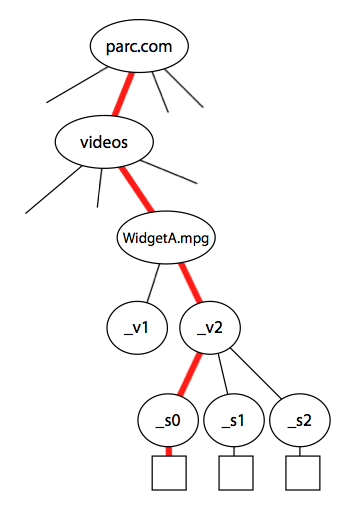
\includegraphics[width=0.4\textwidth]{images/name_tree}
  \caption{名字树遍历} 
  \label{name_tree}
\end{figure}

下面举例说明。图~\ref{name_tree}~中展示了名字树中与图~\ref{name}~关联的部分。如果一个应用程序想要展示最新版视频,它就会表达这样一个兴趣:~\url{/parc.com/ videos/WidgetA.mpg}~\emph{RightmostChild}。在发送方就会执行如图~\ref{name_tree}~中高亮的遍历,
\renewcommand\baselinestretch{1} %调一下脚注行间距
\footnote{默认的遍历规则是\emph{LeftmostChild}}
找到该视频的第二个版本的第一段。一旦这份数据被找到了,数据接收方只要发出带有同一名字外加~\emph{LeftmostRightSibling}~注释的兴趣包即可获得后续分段。另一个办法是接收方直接计算出~\_s1~部分的名字,因为分段规则是由应用程序制定的,不是由~CCN~制定的。

正如前面例子所展示的,数据命名规则可以根据数据包的相对检索特性而专门设计。应用程序可以通过遍历树发掘存在数据。虽然这些都不属于~CCN~基本传输,但是他们都是~CCN~应用程序设计的重要组成部分。我们期待着一大批可重用的习惯的出现,期待着它们被标准化,期待着它们以共享函数库的方式实现,给应用程序开发者提供高度抽象化的模块(如文件和流媒体的传输)。

兴趣包提供了一种对已有数据的限制性查询机制。它是为高效表达接收方的下一个需求而设计的。在这里我们没有足够的篇幅去赘述我们正在研发的查询选项(query options)的细节。不够我们申明用兴趣包限制数据发布者的输出是可以做到的,不需要将整个数据集或整棵子树都发送出去。在简单排序不够用时,兴趣包还可以排除(exclude)已经收到的包。我们还在研发更高级的名字发掘机制。这些机制可以有效发掘大型子树而不一定要取得内容。

%...............................................................%
\subsection{高连通性,移动性及策略}
\label{sec:3.3}

今天的计算机通常都有多个网络接口和极强的移动性。由于~IP~只能在生成树上转发包,它很难利用多网络接口的优势,也很难适应高移动性给网络带来的变化。%为什么呢
~CCN~包不能转发成环,所以~CCN~充分利用多网络接口优势。%为什么呢
~CCN~谈论数据,而不是对节点谈话,所以它不需要把第三层的身份信息(如~IP~地址)和第二层的身份信息(如~MAC~地址)绑定在一起。即使是在连通性快速变化的情况下,~CCN~总是能够快速传输数据——物理传输有多快,~CCN~就能做到多快。再者,由于~CCN~的兴趣包和数据包是配对的,每个节点都可以获得每个名字前缀、每个~face~的细粒度性能信息。这些信息可用于动态将名字和~face~匹配(详见~\ref{sec:6.3})。
\renewcommand\baselinestretch{1} %调一下脚注行间距
\footnote{在~IP~中,路由的不对称性通常决定了中间接地啊不可能知道某一个接口是否真的工作良好,因为路由只能看到一个对话的一个方向。}

正如~\ref{sec:2}~中说的一样,~CCN~特意用与~FIB~表项对应的~face~列表模拟了多连通性。由于缺乏能使用所有~face~的万金油式策略,设计的初衷是让每个~FIB~表项都包含一个程序。这个程序像一台抽象机器,专门负责决定怎样转发兴趣。这台机器的“指令”应该包含普通存取、算术、比较指令的子集,包含一些动作(\emph{sendToAll, sendToBest, markAsBest})和触发器(\emph{interestSatisfied, interestTimedOut, faceDown})。与此匹配的,~face~会有一套开放式的属性(\emph{BroadcastCapable, isContentRouter, UsageBasedCharging, PeakUseLimited})。使用动作,属性可以被动态创建。

这些动作、触发器和属性合并在一起统称策略层(CCN Strategy Layer)。~FIB~表项中的程序就是获得这个表项所指数据的策略。我们目前的默认策略是先给所有具广播能力(\emph{BroadcastCapable})的~face~发兴趣包,如果没有回复,则依次尝试所有其它~face。本地数据(如一场报告中报告人机器中的数据,一次商业会议中同事电脑或手机中的数据)可以直接获得。只有在本地找不到的数据才会使用路由机器去获取。

\begin{figure}[htbp]
\begin{center}
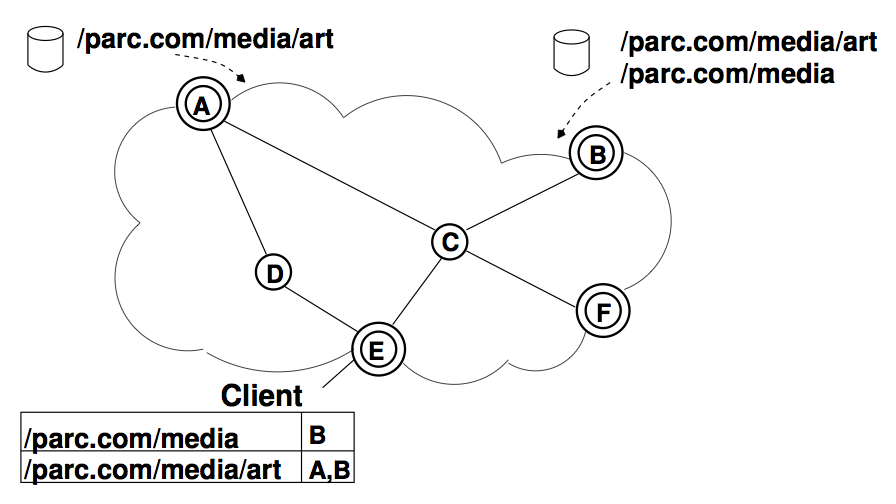
\includegraphics[width=0.7\textwidth]{images/routing}
\caption{将兴趣包路由至域内多媒体内容存放处}
\label{routing}
\end{center}
\end{figure}

FIB~表项中的~face~信息可以通过各种方式获得。如图~\ref{routing}~中的数据源可以用~\emph{Register}~动作作用于本地~CCN~内核,接收对它可以提供的数据的兴趣。这么做会在本地~FIB~表中创建起相关兴趣的表项,并且会在它们后面填上对应程序的~face。已注册的名字会有一个标志位,决定它们是否应该被宣传到本地机器之外。宣传代理(announcement agent)扫描本地注册名字表,把负责他们要求的、被置位了的名字广而告之(详见~\ref{sec:5.4})。本地扫描可以使用局限于本地名字空间的正常~CCN~兴趣包和数据包来做。广告可以使用~CCN~(即让宣传代理提供~\url{/local/CCN/registrations}),可以使用标准~IP~服务位置协议(SLP),或使用~CCN~或~IP~路由(详见~\ref{sec:4})。%不确定

%===========================%
\section{路由}
\label{sec:4}
近年来路由在学术研究领域的热度回升。今天大多数路由问题都有了许多有趣且有效的解决方案。所有对~IP~奏效的路由机制都应该对~CCN~有效,因为~CCN~的转发模型是~IP~模型的严格超集。~CCN~转发模型有更少的限制(不为了避免成环而禁止多数据源、多目的地传输),并且路由语义(结构化名字集合与最长匹配)也与~IP~的转发模型相同。~CCN~为路由协议的传输提供了一个极佳的交通工具:大多数路由传输协议的核心是一个与~CCN~的内容为心、有引导的弥漫扩散模型极为相似的东西。此中原因是它们的工作时间都在网络的拓扑期之前,这时候对等体双方的位置和身份都还未知。由于~CCN~是一个文件的信息安全模型(详见~\ref{sec:5}),使用~CCN~进行路由传输即可自动完成路由保护。

为了解释如何将~CCN~映射到路由机制中去,~\ref{sec:4.1}~描述了~CCN~将如何使用未经任何修改的互联网链路状态内部网关协议(IS-IS或~OSPF)路由。这既是为了展示~CCN~如何使用现有常规路由方法,
\renewcommand\baselinestretch{1} %调一下脚注行间距
\footnote{现有传统路由方法是相对于那些以内容为导向的路由方法(如~Small Words)而言的。那些方法也可应用于~CCN,但是采取的策略完全不同。}
又是为了说明~CCN~与~IP~的兼容性极好,使用现有的基础设施即可大范围使用。
% EGP外部网关协议
% IGP内部网关协议
%  |-- 距离矢量路由协议
%  |-- 链路状态路由协议(IS-IS, OSPF)
%  |-- 混合路由协议

%...............................................................%
\subsection{链路状态域内路由}
\label{sec:4.1}
域内路由协议为节点提供了发现和描述本地连通性(邻接性)和描述直接连接着的资源(即宣告的内容)的途径~[17, 16]。这两种方法是正交的——一个描述图中的链接,另一个描述图中节点的拥有的资源。这两个操作常常在完全不同的信息域中完成。比如,~IS-IS [17]~用~IEEE 802.1~第二层的物理地址描述连通性,而使用第三层~IP4~或~IP6~前缀来宣告内容。如~\ref{sec:2}~中所说的,~IP~转发和~CCN~转发基本上是相同的。它们都使用基于前缀的最长匹配(而且使用的理由也一样——结构化的细节集成)来找拥有更接近于辨识标志的邻居。既然两个~FIB~有诸多相似之处,读者可能会猜想那些用于创建~IP FIB~的设备也许可以轻松地被改造成为创建~CCN FIB~的设备。事实正是如此。

CCN~前缀与~IP~前缀是不同的,所以主要的问题是它们是否可能被一些路由协议描述和表达。幸运的是,~IS-IS~和~OSPF~都可以用一个通用的类型标签值(TLV, type label value)机制~[18, 19]~来描述直接连接的资源,并且这个机制对于传播~CCN~内容前缀也很合适。此机制的明细中说,无法识别的类型应该被忽略。这就是说实现~CCN~全套转发模型的路由可以直接依附到现存的~IS-IS~或~OSPF~网络中去,无需改动现存网络或者它的路由。内容路由通过邻接协议学习到网络物理拓扑结构,并在那个结构中宣告自己的位置。路由还可以通过~CCN TLV~机制来宣告内容。

举个例子,图~\ref{routing}~展示了一个含有一些(单周期)~IP~专用路由和~IP CCN~复合路由的内部网关协议(IGP)域。靠近~A~的一个多媒体仓库正在(通过向本地网络管理名字空间发送广播的形式)宣告它可以为与前缀~\url{/parc.com/media/art}~匹配的兴趣包提供服务。~A~中的路由程序听见了这个宣告(因为这个路由程序已经对其名字空间内的这类宣告表达过兴趣),于是它就在本地~CCN FIB~为此前缀新建一个表项,在~face list~中填上它收到宣告的那个~face。这个路由程序随后把这个前缀封装为~IGP LSA。这样这个前缀就扩散到网络所有节点。当网络中的其他路由程序,比如说~E~中的路由程序,首次得到这个~LSA~时,它会新建一个到~A~的~CCN face,并在本地~FIB~中添加~\url{/parc.com/media/art}~一项,~face list~写~A。当一个靠近~B~的仓库宣告~\url{/parc.com/media}~和~\url{/parc.com/media/art}~时,~B~也将这两个前缀的~IGP LSA~扩散出去,其结果是~E~的本地~CCN FIB~会如图~\ref{routing}~中所示的那样。如果~E~的附近有客户表达~\url{/parc.com/media/art/impressionist-history.mp4}~这样的兴趣,这个兴趣会向~A和B~转发,而~A~和~B~则各自发送给自己附近的多媒体仓库。%名词未考证

CCN~动态创建对于带宽和延时而言近似最优的拓扑结构。数据至向有兴趣存在的地方流动,且选择最短的路径。对于任何一份数据,任何一个连接中至多只有一份它的副本经过。然而这种递送拓扑目前显然不是最优的,因为如果靠近~F~的客户也对同一部电影感兴趣的话那么同样内容的第二个副本又必须流过~A-C~连接或~B-C~连接。这种情况发生的原因是在~CCN~部署过程中有很多拓扑结构对于~CCN~而言不可用(C不是内容路由,所以它不会缓存数据)。一旦~C~进行了~CCN~软件升级,~E~和~F~就会通过它来转发兴趣,那么传输就是最优的了。%名词未考证

在上面讨论过的模型中,~IGP LSA~被使用于传输含有完整的~CCN~验证、保护和政策注释的标准~CCN~信息。因此即使~IGP~是不安全的,存在于具有~CCN~能力的节点间的通信也是安全的。如果所有节点都具有了~CCN~能力,那么~IGP~拓扑结构自然就安全了(详见~\ref{sec:5.1})。保障外界产生的前缀布告的安全性也是宣告协议的功能之一。~CCN~内容前缀,如图~\ref{routing}~中媒体服务器宣告的那些,有稳健的信任模型,并由~CCN~保障其安全性。外界~IGP~或~BGP(边界网关协议)~产生的~IP~前缀将不被信任。

当存在多个同一前缀的布告时,~IP~和~CCN~之间存在行为差异。在~IP~网中任何所有节点都会把所有匹配的通信量送到一个宣告者那里去。在~CCN~网中所有节点会把所有匹配的兴趣包发到所有宣告者那里去。这一行为差异的根源在于语义差异:从某个~IGP~路由来的~IP~前缀布告会说“所有带有这个前缀的主机都可以通过我访问到”;与之等价的~CCN~布告会说“一些带有这个前缀的内容可以从我这里访问到”。由于~IP~没有办法在内容层面上防止成环,它只好去建设无环转发拓扑结构,即一个以目的地为根节点的汇点树。由于一棵树中的任意两节点间只有一条路径,一个~IP FIB~表项只有一个用于存放输出接口的空位。于是所有与某个前缀关联的主机都必须通过发出布告的这个节点才能访问,因为所有的通信量都被送到那里去了。由于~CCN~包无法成环,一个前缀布告不需要保证某一节点与前缀所能表示的所有内容都相连,且~CCN FIB~也被设计成将兴趣转发至宣告过前缀的所有节点。这一语义变迁可以在不改变~IGP~的前提下完成,因为这是实现上的变化,不是协议上的变化。~IP~要计算从前缀宣告计算生成树,~CCN却不要。~CCN~是在信息消费处计算,而不是在信息生产处计算,所以它和~IP~最终收到的信息都是完整的。
\renewcommand\baselinestretch{1} %调一下脚注行间距
\footnote{严格地说,这句话对链路状态内部网关协议如~IS-IS~和~OSPF~是正确的,但对距离矢量协议如~RIP~和~EIGRP~却不正确。后者的路由公告涉及到~Bellman-Ford~计算,预测生成树并抑制其它连接。这样的~IGP~就需要稍稍改动一下文中所述的机制了。}

%...............................................................%	
\subsection{域间路由}
\label{sec:4.2}
一旦一个互联网供应商(ISP)的一部分客户开始使用~CCN,ISP~就最好开始部署内容路由器以节省成本(一份数据不管有多少用户需要,都只需要从互联网供应商的连接中走过一次)和降低客户平均延时(一份数据的多个副本除了第一份之外均来自互联网供应商的本地内容存储库)。因此,一旦~CCN~的部署冲破一个基线以后,它就会自底向上地,以一种激励性的方式迅速成长。由于用户直接与他们的供应商相连,他们没有必要借助一个服务发现协议来了解供应商的内容路由。这类协议可以把~CCN~注册公告(详见~\ref{sec:3.3})当做通配符(零前缀),或者使用任拨(比如所有内容路由的~IP~地址都设为~10.0.96.95),~DNS~惯例(如所有内容路由都使用~\emph{ccn.isp.net}~域名),~DNS SRV [14],~SLP [15]~等等。这些选项都不要求传播任何内容前缀。

这样自底向上的部署方法最大的问题在于跨越被无内容路由~ISP~分割的有内容路由域之间的鸿沟。比方说一个位于~\emph{parc.com}~的内容路由想要前缀为~\emph{mit.edu}~的内容,然而~PARC~与~MIT~之间并无内容路由器。使用此前缀进行一个(启发式的)~DNS~查找,确定位于~MIT~的内容服务器(群)的~IP~地址(或通过~\emph{\_ccn.\_udp.mit.edu} SRV~查找,或进行~\emph{ccn.mit.edu}~地址查找),可以自动地、按需地建立起连接两个内容服务器的基于~UDP~隧道的~face。然而当鸿沟并不位于两个域的边缘时,这一机制就工作得不那么理想了。如果~PARC~和~ISP~的供应商都提供内容路由服务但是它们却由不支持~CCN~的供应商连接,~PARC~的供应商就无法获知~MIT~的供应商那里的相关路由,于是它就会把兴趣包发送到~MIT。因此若不添加额外机制,~ISP~路由器照顾了进口内容(被它的客户要求过的内容),却没有照顾到出口内容(它的客户生产的内容)。这在一定程度上削弱了~CCN~的一个主要的长期优势,即令内容传播树根节点处的通信量与内容流行程度无关。今天,这个通信量仍在随着流行程度增长(详见~\ref{sec:6.2})。

这一问题可以通过把域级内容前缀整合入边界网关协议(BGP)来解决。目前的~BGP~域间路由已经有~IGP TLV~的等效机制,允许域广告其客户的内容前缀。~BGP~的~AS-path~信息亦可以使各个域建立起在自制系统层面上的而非网络前缀层面上的拓扑地图。这个地图在功能上与~IGP~建立的地图等效(它使人获知提供某个前缀的域,以及通向这些域的最短路径上有哪些具有~CCN~能力的域),所以算法可以通用。


%===========================%
\section{内容为心安全}
\label{sec:5}
CCN~建立在基于内容的安全之上:保护和信任与内容一路随行,不是内容经过的连接的一种属性。在~CCN~中,所有的内容都由数字签名验证;私密内容由加密算法保护。这是~CCN~动态内容缓存机制的一层重要保障——如果你将要得到一份离你最近的数据副本,你必须能够验证你得到的数据。目前的~IP~网络根据内容从哪里来和内容是怎样得到的来决定是否信任内容,因此客户必须从原始数据源那里直接获取内容。使安全与内容融为一体可以减少我们在网络中间环节的忧虑,从而开放网络获得广泛参与。在这个章节中,我们给出~CCN~核心安全设计的总览,并强调其中的新颖之处。详细的分析,包括撤销之类的话题,都要在另一篇文章中讨论。额外背景和研究动机在~[34]~中描述。

%...............................................................%
\subsection{内容验证}
\label{sec:5.1}
CCN~验证名字与内容之间的绑定。每个~CCN~数据包的签名(如图~\ref{packet_types})都是对该数据包的名字、内容和少量对签名验证有帮助的辅助信息(图~\ref{packet_types}~中的~signed info)进行的。这使内容发布者可以安全地将任意名字与内容绑定。与此形成对比的是,此前的许多方法为了安全,都要求名字能够自认证(self-certifying),如使用内容的加密摘要作为它的名字~[16, 28, 12, 9]。直接使用对用户或对应用程序有意义的名字的能力增强了可用性,简化了传输。没有这种能力的系统将需要一个“间接设备(indirection infrastructure)”~[4, 6]~把人们关心的名字映射到安全的、不透明的、自认证的名字上去。这样的系统的安全性就受那个(常常是不安全的)间接设备的限制。

CCN~数据是可以公开验证的——每个数据包的签名都是标准的公钥签名,并且通信流上的任何机器(包括端点和沿路的所有机器)都可以验证一个名字和内容的绑定是否是用某个公钥签署的。签名算法是有内容发布者从一个大的确定的集合中根据某一数据的性能要求选择的——比如要求验证数据最少,或要求签名的生成和验证的延时和计算成本最小等。虽然数据包都被设计为单独验证,我们仍然可以用像~Merkle Hash Trees [27]~这样的集成办法降低计算成本。

每个签了名的~CCN~数据包都含足够的信息使人能够以此获取到验证此包的公钥。它的支持信息中包含有那个公钥的加密文摘。它可以作为数据发布者的一个简短辨识符号,也可以帮助验证者快速地从本地缓存中找到那个公钥。包中还含有一个钥匙定位符,指示了获得公钥的方法;它可能是公钥本身,也可能是能够用于获取公钥的~CCN~名字。

CCN~最底层的内容验证完全是语法上的验证——它只是确认一下内容是由它声称的那个公钥签署的。它并不给那个公钥赋予任何实际意义——它属于谁,它所签署的数据是否应该被用户信任。即便是这样一点微不足道的验证工作也是很有用的,尤其是在防御多种网络攻击的时候。例如,这使得内容消费者在申请数据时既指定内容的名字又指定内容的发布者,这样他们就可以在有虚假恶意信息存在的情况下仍然得到他们想要的信息。~CCN~的路由器可以选择全验证、部分验证或不验证它们经手的数据包,这视它们的资源数量而定。它们还可以根据是否检测到网络攻击动态地决定是否验证更多的数据。

%...............................................................%
\subsection{信任管理}
\label{sec:5.2}
虽然~CCN~以点对点形式传输数据,它却在数据发布者和数据消费者之间提供端对端的安全。~CCN~内容消费者必须决定收到的内容是否是值得信任的。在~CCN~中信任的概念是上下文相关的,即它是由内容的上下文和内容的用途决定的。比如,我们可能需要一份法律文件由被法庭授权的人签署,一篇博文则只需要签上与这个博客里的其他文章一样的签名就可以了,有时可能连这个要求都不需要达到。这种方法较万金油式的信任管理办法(比如认定数据发布者非黑即白)更为灵活易用。

基于内容的安全的基本原语——经验证的从名字到内容的绑定——可以用来实现更高级的信任机制。~CCN~签名绑定机制的本质作用是认证内容。当名字指代一个组织或个人,且内容是一个公钥时,这就是一个数字证书。这使~CCN~能够很容易地支持传统的密钥信任建立机制。更有趣的是,通过允许内容安全链接到另一个内容,我们就可以用内容去认证内容。这样我们就可以把对少量密钥的信任转化为对一群互相关联的内容的信任。

% . . . . . . . . . . . . . . . . . . . . . . . . . . . . . . . %
\subsubsection{公钥信任}
\label{sec:5.2.1}
应用层面的~CCN~消费者必须面对传统的密钥管理问题——将公钥与个人和组织相关联(因为通常情况下都是这些现实生活中的身份信息在决定谁是一个内容的可信签署者)。~CCN~从几个方面将此任务简化了:第一,它直接、简单地解决了获取公钥这个实际问题。密钥只是另一种形式的~CCN~数据;~CCN~简单的命名习惯确保了它们能够容易地被找到。

第二,如上文所说,只需要把公钥作为~CCN~内容发布就相当于为公钥生成了一张证书——~CCN~名字和那个公钥的绑定是由发布者(签名者)认证的。这个积木式部件可以来表示任意密钥之间的信任关系——从简单的树(如传统的公钥基础设施,~PKI)到任意的图(如加密隐私信任网~PGP Web of Trust)。

第三,~CCN~不强制使用任何普适的信任模型。信任是内容发布者和消费者之间的事。对一个应用程序合适的可能对其它程序并不合适。用户可以自由使用现存的公钥信任模型(如~PKI),或者自定义新的适合~CCN~使用的模型。

SDSI/SPKI [32, 10, 2]~的模型就特别适合~CCN~使用。在这个模型中公钥和现实身份由本地控制的命名空间映射。比如一个组织的成员的公钥如果被这个组织所证明,那么这个成员就可以被承认,无需通过外界第三方来证明(如~Verisign)。知道了~\url{parc.com}~的公钥,我们就可以验证公司员工的公钥。更进一步,如果我们信任~\url{parc.com}~的一个员工,那么我们可以去他的~SDSI~名字空间查看~\url{parc.com}~的身份和公钥。使用一些用户友好的机制(如个人通讯录,组织成员名单,公众经验等~[30, 37]),我们可以得到一个公钥已经验证的用户集合。从这个很小的集合出发,我们可以用~SDSI~模型推演出一个我们信任的内容发布者的大集合。

我们可以将~SDSI~身份直接映射为~CCN~名字,并且直接在~CCN~内容里表达~SDSI~信任关系。这样的名字空间树可以组成一片森林——一个内容消费者可能会相信她拥有~\url{parc.com}~(或者~\url{/parc.com/george})的真实公钥;她这么相信的原因可能是由于她的亲身经历(比如她是~PARC~的一个员工),可能是基于她的朋友提供的信息,也可能是由于此公钥出现在受信任的公钥目录中。~CCN~不要求,甚至不预想这些树有一天会像它们在传统的全球商业~PKI~中一样聚集成一棵(或只有少数几个根节点)。最值得注意的是,是消费者们根据各种信息决定他们为什么要信任一个公钥,而不是依靠发布者们从某一个商家那里获取一个证书。

\begin{figure}[htbp]
\begin{center}
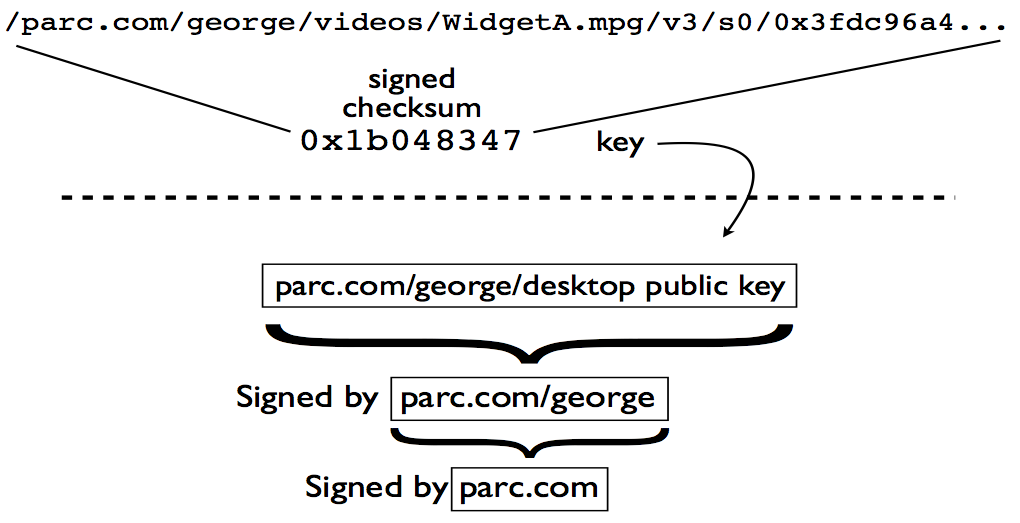
\includegraphics[width=0.7\textwidth]{images/trust}
\caption{CCN~信任建立模型可以将内容空间与发布者密钥相关联}
\label{trust}
\end{center}
\end{figure}

另外,通过把内容组织在层次化的名字空间里,~CCN~可以把签名政策甚至是公钥与特定的名字关联起来;一个层级的名字空间可以由它的上一级来签名认证。如图~\ref{trust}~所示,~\url{parc.com}~的密钥认证了用户~\url{george}~的密钥;这个密钥又认证了~\url{george}~那台桌面电脑的密钥。这些以~CCN~数据形式存在的信任宣言可以帮助消费者评估此发布者究竟是不是~\url{WidgetA.mpg}~的可靠发布者。

% . . . . . . . . . . . . . . . . . . . . . . . . . . . . . . . %	
\subsubsection{基于证据的安全}
\label{sec:5.2.2}
我们可以在结构化名字的概念中添加安全引用(secure reference)一词。它与受信任的超链接或书签很相似。一个~CCN~内容不仅可以使用名字来引用另一个内容(引用目标),它还可以使用加密文摘(加密文摘在功能上也是一种能够自认证的名字~[26, 28, 12, 9])或使用内容发布者的身份信息(密钥)来引用~[9, 31, 25, 24]。这样的引用可以用来表达委托(delegation)的概念。比如一个数据发布者~$P$~发布了一个名为~$N$~的链接,引用目标为~$(N' , P')$,这意味着链接发布者~$P$~希望~$N$~指代~$P'$~发布的~$N'$~的引用目标。

这样的引用引用引用可以表达传统形式的委托,也可以用于建立一个内容信任网络——经签名认证的内容个体有效地认证它们安全连接到的内容,组成一张网络。比如如果用户决定了信任一个名为~$A$~的网页,那么他就可以自动地信任由~$A$~安全连接到的内容,如它的图片、广告、原材料等等,不需要额外的管理和设置。这样的信任的粒度是极细的——那些材料只是在~$A$~的上下文关系下才被认可。

用户遇到的每一个内容都是它的引用目标的可靠性的一个潜在证据。如果很多我们信任的发布者都说它们信任~$P'$~给出的~$N'$~的值,那么我们就更有可能相信这个值。如果一个黑客袭击了一个发布者,比如获取到了~$P''$~的私钥并用它伪造了一个~$N'$~的值,这样的攻击将不会奏效,因为大多数证据仍然指示出了正确的值。每增加一份可信的签名证据,这样的黑客袭击就会难上加难,因为袭击者是无法销毁所有证据的。

%...............................................................%	
\subsection{内容保护与访问控制}
\label{sec:5.3}
控制~CCN~内容访问的首要方法是加密。~CCN~不强制受信任的服务器和目录使用访问控制协议;不管是谁得到了私密的内容,只有经授权的用户才能解密。

对数据、名字、名字部件的加密都是对网络完全透明的——对~CCN~而言,它们都不过是二进制数据而已(尽管出于路由的高效性和数据排序的角度考虑一些名字部件最好是明码)。解密密钥可以以~CCN~数据块的形式和它们的内容一起传播。封装在用户友好的函数库中的命名习惯可以使查找解密密钥的任务变得容易。~CCN~不强制使用任何加密机制或密钥配送机制——用户只需要为一个内容确定编码传播解密密钥的方式就可以建造起自定义的、面向应用程序的访问控制模型。

%...............................................................%	
\subsection{网络安全与策略实施}
\label{sec:5.4}
CCN~的设计使它免受多种网络攻击的侵扰。对包括路由信息和策略信息在内的所有内容实施认证防止了数据被仿冒和篡改。~CCN~消息只能谈论内容不能对主机说话这一实施使得向特定目标发送恶意包变得非常困难。针对~CCN~网络的攻击为了奏效,只能专注于拒绝服务攻击(denial of service):把合法内容“隐藏”起来(如故意不返回可用的新版数据)或使其沉没——制造海量假数据包阻止真数据包的递送。

为了确保消费者在可能有大量仿冒数据存在的情况下能够得到他们需要的数据,消费者们可以对能满足其兴趣的数据发布者提出限制条件。现有的限制条件力争在网络传输效率和对于消费者的易用性之间取得平衡。至少,消费者(或代表消费者利益的软件)可以指定他们需要的数据必须由特定的发布者(公钥)签名,或由一个已认证了发布者的公钥的密钥签名。这层间接关系避免了那些需要内容消费者通过推理演绎得知签署内容的密钥的系统的脆性。

CCN~吸收整合了一些防止无用通信过度转发的机制。兴趣包和数据包之间的流平衡防止了数据在本地链路之外泛滥的强力拒绝服务攻击(brute force denial of service)。流平衡存在于跳与跳之间。只有下行兴趣包要求的数量的数据包会被发过一个链路。即使一个兴趣包被发到很多个网络中去寻找数据包(这不太可能发生,但是要根据路由情况而定),在每一个汇聚点只有一个数据包会被发送到内容消费者那里去。基于数据的分布式拒绝服务攻击是不可能发生的。

由于消费者可以自行选择生成数据包的速率,从理论上来说消费者有可能制造基于兴趣的泛洪攻击(Interest flooding attack)——分布式地生成海量数据包,以图吞噬~CCN~路由器认为通向潜在数据源的全部可用带宽。多个申请同一数据的兴趣包会被~CCN~路由合并,只有一个兴趣包会被转发至上行。因此,为制造一次兴趣泛洪攻击,攻击者生成的大量兴趣包的名字必须有共同的前缀(攻击目标)和不重复的名字部件(以防止兴趣被合并)。由于~CCN~机制允许传输关于尚不存在的内容的兴趣,这些兴趣包通常会被转发到它们的目标。

CCN~的两个性质可以帮助抵抗这种攻击:第一,由于数据包会沿着它们满足的兴趣包的路径原路返回至消费者处,每一个~CCN~中间节点都可以清楚地知道它所转发的每一个兴趣最后是否成功获取到了数据。(这在~IP~网络中就不成立,因为转发和返回路径常常是不同的。)随机生成的兴趣洪泛包一般是不会得到回复数据的。一个简单的适应性算法就可以使中间路由器根据带某个前缀的兴趣包的成功率(取回数据率)设置对应兴趣包的转发数量上限。第二,受攻击的域可以要求下行路由器紧缩来自特定名字前缀的兴趣包的数量,这类似于~IP~网络可能会要求它的上行节点紧缩对于未使用的地址的访问。不过,~CCN~将政策与名字空间绑定的能力将允许它做出选择性的控制。

CCN~还提供工具使公司或组织能对他们的内容的传播范围加以控制。属于一个组织或服务供应商的路由器可以实施基于政策的路由(policy-based routing),即内容的路由政策是和名字及签署者相关联的。一个简单的例子是一个”内容防火墙”,它只允许申请~\url{/parc.com/public}~名字空间下的内容的兴趣包被满足。一个组织可以发布政策,规定什么密钥可以签署那个名字前缀下的内容(如:所有的密钥都须由~\url{ccnx.org}~签署),并要求它的内容路由器在发现某内容不满足此要求时自动终止对它的路由。这些路由器本身并不需要理解此事件涉及到的名字和组织等语义。最后,在一些情况下兴趣包还可以被数字签名,使得政策路由可以限制申请者的名字空间和申请频率。

%===========================%
\section{评估}
\label{sec:6}
本节中我们对我们实现的~CCN~原型的性能进行了描述和评价。在目前的实现版本中我们用基于字典的标签压缩法将数据包进行了~ccnb~精简二进制~XML~表示。我们的~CCN~转发器~\url{ccnd}~是用~C~实现的。它将作为一个用户空间的守护进程。兴趣包和数据包被封装在~UDP~包中,以便利用现存的网络通过广播、多播和单播转发。

大多数使用~CCN~的机制(~\url{ccnd}~通信,密钥管理,签名,基本加密解密和信任管理)都体现在一个~CCN~函数库中。这个用~Java~和~C~写成的函数库封装了处理名字和数据常用惯例,如名字中分片和版本号的编码方式,又如重现密钥信息以利加密和信任管理。这些管理被组织成配置文件(profile)的形式,重现了面向应用程序的协议,位于~CCN~基本兴趣数据协议之上。

这样的结构有蕴含两层含义。第一,敏感数据的安全警戒线被推至应用程序中;内容只在有权知情的应用程序中被解密,永远不会在操作系统的网络栈或硬盘上被解密。第二,使用~CCN~的应用程序需要做很多关于名字和数据惯例的协商,使生产者和消费者意见统一。

\def\tm{\leavevmode\hbox{$\rm {}^{TM}$}} %注册符 网上找的
所有模块均可在~Linux, Mac OS X\tm, Solaris\tm, FreeBSD, NetBSD~和~Microsoft Windows\tm~中运行。加解密操作由~OpenSSL~和~Java~提供。

%...............................................................%
\subsection{数据传输的效率}
\label{sec:6.1}
TCP~很擅长传输数据。对于批量数据的陆上传输,~TCP~的常规应用到应用递送吞吐量可以接近理论上限(瓶颈链路的带宽)。~TCP~可以“把管道填满”,因为它的可变大小的窗口可以容许足够多的数据被传输,去填满沿途带宽与延时的乘积和途中所有存储转发缓存空间~[21]。~CCN~能够同时保持多个兴趣的能力(详见~\ref{sec:3.1})赋予了它相同的能力。我们认为它的数据传输性能是与~TCP~的类似的。

为了检验这个观点我们测量了在不同~TCP~窗口和~CCN~兴趣数量下传输~6MB~文件所需的时间。测试是在两台用~100Mb/s~连接接入校园以太网的~Linux~主机之间进行的。在对~TCP~的检测中我们使用~ttcp~传输文件。在对~CCN~的检测中,我们先在数据发送方本地请求一次数据,把文件预装进~ccnd~的内容仓库。
\renewcommand\baselinestretch{1} %调一下脚注行间距
\footnote{这么做的原因是使测量结果仅包括传输时间,不包括为~CCN~内容签名所消耗的时间。}
其结果是制造了~6278~个拥有自己的名字的签过名的~CCN~内容,每个内容有~1 KB~的数据量(内容总大小约为~1350~字节)。

\begin{figure}[htbp]
\begin{center}
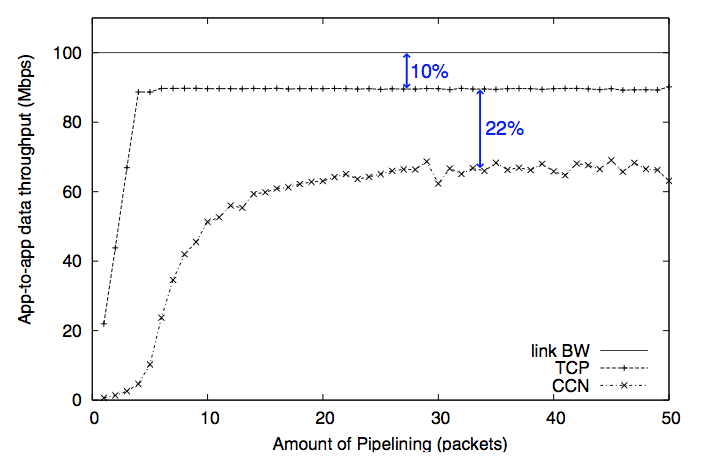
\includegraphics[width=0.7\textwidth]{images/performance}
\caption{批量数据传输性能}
\label{performance}
\end{center}
\end{figure}

测量结果见图~\ref{performance}。
\renewcommand\baselinestretch{1} %调一下脚注行间距
\footnote{由于~CCN~是以一个包大小的内容为单位传输,图中的~TCP~窗口大小也被除以了每个包的数据量,转换成了包的数量。}
CCN~需要~TCP~五倍的流水化程度(4~包比~20~包)才能达到~TCP~吞吐量的渐近线。但这其实是一种假象:我们的原型是在应用程序的层次上实现的,其执行完全未加优化,会有额外的存储转发环节被引入;~Linux TCP~则是在内核中被实现的,并且是高度优化了的。~TCP~吞吐量可以达到链路带宽的~90\%,这个比例体现了它的包的头部开销(净荷与包大小之比)。~CCN~能达到链路带宽的~68\%。由于在这个测试中~CCN~被封装在~IP/UDP~中测试,它具有~TCP~的所有开销,外加~22\%~它自己的头部开销。因此对这个例子而言~CCN~的批量数据传输效率与~TCP~处于同一数量级,但由于其头部更大,传输效率比~TCP~低。
\renewcommand\baselinestretch{1} %调一下脚注行间距
\footnote{CCN~包相对于~TCP~包的头部体积增长是出于增加了很多安全注释(如签名、公钥定位符等)。}

批量数据传输性能对于下载大型多媒体文件这样的任务是很重要的,不过用户对于网速的体验更多地取决于网络传输体积小很多的网页内容的速度。我们比较了~CCN~和~HTTP、HTTPS~获取单个~HTML~文件的速度。在非安全(HTTP)案例中我们使用了~Google~的主页,在安全(HTTPS)案例中我们使用了~Wells Fargo~银行的主页。有两种~CCN~封装方法被测试:直接封装为~1500~字节的以太网包(无~IP~或~TCP~头部,净荷域~1230~字节),或封装为~UDP~数据报(最大净荷~7656~字节)。
\renewcommand\baselinestretch{1} %调一下脚注行间距
\footnote{由于这些数据报大于~1500~字节的路径最大传输单元,它们将被~IP~分割。对包数和字节数的统计包括了这些分片及分片头。}

{
\renewcommand{\arraystretch}{1.2}
\renewcommand{\tabcolsep}{0.2cm}
\begin{table}[htdp]
\begin{center}
\begin{tabular}{|c|c|c|c|c|}
\hline
\space & \multicolumn{2}{c|}{Bytes (packets)} & \multicolumn{2}{c|}{Overheads}  \\
\space & Sent & Received & Encap & Transact \\
\hline
\multicolumn{5}{|l|}{Web Page (6429 bytes)} \\
\hline
HTTP & 723 (9) & 7364 (9) & 15\% & 11\% \\
CCN/ETH & 811 (8) & 8101 (6) & 26\% & 13\% \\
CCN/UDP & 325 (3) & 6873 (5) & 7\% & 5\% \\
\hline
\multicolumn{5}{|l|}{Secured Web page (16944 bytes)} \\
\hline
HTTPS & 1548 (16) & 21232 (22) & 25\% & 9\% \\
CCN/ETH & 1791 (16) & 20910 (14) & 23\% & 11\% \\
CCN/UDP & 629 (5) & 18253 (14) & 8\% & 4\% \\
\hline
\end{tabular}
\caption{网页内容传输效率}
\label{web_performance}
\end{center}
\end{table}
}

结果汇总见表~\ref{web_performance}。前两列给出了获取一个~HTML~文件过程中收发总字节数和包数(包括所有用于控制的通信量如~SYN~和~ACK~包)。后两列是由前两列计算得出的,给出了每种协议的开销比例:~Encap~测量了数据封装的开销,它是开销字节数(收到的总字节数减去收到的数据字节数)与数据字节树之比;~Transact~测量了会话开销(请求一份内容的成本),它是总发出字节数与总收到字节数之比。

由~CCN~传输内容总是安全的,不过测试的结果显示了~CCN~的性能与无安全保证的~HTTP~相当,比有安全保证的~HTTPS~好很多。位于以太网之上的~CCN~和~HTTP~效率相等(CCN~每个包的字节数更多但是包的总数较少,即来回次数较少),并且是~HTTPS~效率的两倍(只需一半的包数量)。位于~UDP~之上的~CCN~的传输效率从包数量和开销来说都是~HTTP~的两倍,~HTTPS~的四倍。

%...............................................................%
\subsection{内容传播的效率}
\label{sec:6.2}
前文考量了~CCN~作为~TCP~的直接替代(不考虑数据分享)时的性能。~CCN~的主要优势是它自动、透明地分享数据。它可以达到一个为所有内容服务的网页代理的最佳性能,而且不需要任何预设。

\begin{figure}[htbp]
\begin{center}
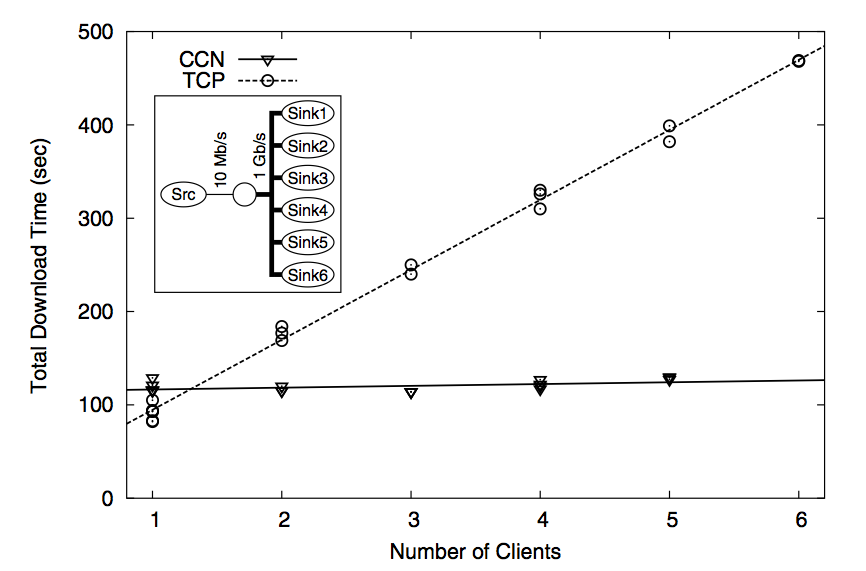
\includegraphics[width=0.7\textwidth]{images/share_performance}
\caption{总下载时间比客户数量}
\label{share_performance}
\end{center}
\end{figure}

为测量数据分享性能我们比较了~TCP~和~CCN~在同一个网络瓶颈面前同时获取多个大型文件所花费的总时间。测试网络参见图~\ref{share_performance}。我们的源节点由一个~10 Mbps~的共享链接连接到一群用~1 Gbps~链接相连的漏节点。
\renewcommand\baselinestretch{1} %调一下脚注行间距
\footnote{虽然我们用的节点很少,但是我们使用了一个~10 Mbps~瓶颈链接来清楚地展示饱和状态下的行为。}
这些机器有各种不同的硬件架构(Intel, AMD, PowerPC G5)和操作系统(Mac OS X 10.5.8, FreeBSD 7.2, NetBSD 5.0.1, Linux 2.6.27)。

所有的漏节点同时向源节点请求一个大小为~6MB~的文件。在~TCP~的测试中这个文件由源机器上的一个~http~服务器提供,由漏机器上的~\url{curl}~程序获取。在~CCN~的测试中这个文件需要预处理(如~\ref{sec:6.1}~中所述)。对于~TCP~和~CCN,我们都记录了最后一个下载完整个文件的节点所花费的时间。我们还更换了漏机器并对同一实验进行了多次重复。

实验的结果如图~\ref{share_performance}。当只有一个漏节点时~TCP~凭借其更小的头部能够比~CCN~更快地完成下载任务。然而随着漏节点数量的增多~TCP~的任务完成时间也线性地增加了,而~CCN~的完成时间则基本不变。请注意,使用~CCN~代替~TCP~会带来~20\%~的性能下降,但与此同时~CCN~的内容分享带来的性能增益则是成倍的,这意味着即使在低分享率、低命中率的环境下~CCN~仍然能够凭借其综合性能战胜~TCP。事实上,这种胜负差距比本实验中展示的更大,因为同样的原理适用于网络中的每一个链接,并且可以完全消除我们现在在受欢迎的交换机和对等体那里经常看到的通信密集的现象。今天,一个热门~YouTube~视频会在~youtube.com~和它的网络服务提供商之间的链路上传输上百万次。如果这个视频是由~CCN~传播的话,那么它只需要经过那个链路一次。在现有的网络架构下,在汇聚点处的通信量峰值会随着热门内容的消费率同时攀升。如果使用~CCN~架构,这个值只会随着热门内容的生产率增长,而今天生产率显著地低于消费率。

%...............................................................%
\subsection{VoCCN~与策略层}
\label{sec:6.3}
为了展示~CCN~支持点对点协议的能力,我们实现了位于~CCN~之上的~VoIP,我们称它~VoCCN。全套细节和性能评估请参考~[22]。在本节中我们以~VoCCN~电话为例展示了~CCN~策略层的行为表现和它的优势。

如~\ref{sec:3.3}~中所述,当~FIB~中一个内容前缀对应多个~face~时,策略层会动态选择最好的一个。可以这么做的原因是:首先,~CCN~可以向多个~face~发出同一个兴趣包(不存在成环的危险);其次,一个~CCN~节点一定可以看到它发出去的兴趣包返回的数据包(不像~IP~网络,请求数据的包和返回数据的包所走的路径可能是完全不同的)。这两个特性使得策略层可以偶尔进行一些实验:一个兴趣包可以被发送到与它的前缀关联的所有~face~中;如果有一个~face~的返回速度比当前认定的最快~face~还要快,那么这个~face~就会成为新的最佳~face~并专门用于转发这个关联前缀,直到下一次实验发生(如收发~200~个包以后,或在载体或~SSID~变化的时候,或当一个兴趣包超时的时候)。
%carrier一词,不是很确定

为了检验这个机制是否正确我们在两台~Linux 2.6.27 (3.4 GHz Intel P4, 2.66 GHz Intel Core2 Duo)~机器上运行了我们的基于~linphone~的~VoCCN~客户端。两台主机分别被连接到两个相互隔绝的~1 Gbps~以太网中。~linphone~默认把音频分割为~20ms~的帧,所以音频活动成为了一个稳定的~50pps RTP~源。
%pps: packet per second
%RTP: realtime transport protocol
从声音质量来衡量,我们的安全的~VoCCN~原型与常规~linphone~性能等同。两个客户都没有包丢失,不过有少量(少于~0.1\%)的~VoCCN~包因晚到而被丢弃。

\begin{figure}[htbp]
\begin{center}
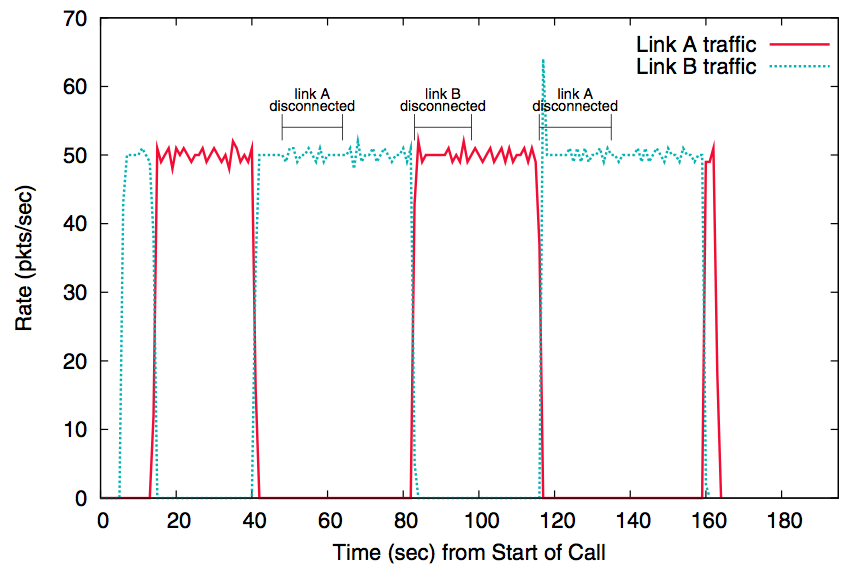
\includegraphics[width=0.7\textwidth]{images/failover}
\caption{CCN~自动失效接管}
\label{failover}
\end{center}
\end{figure}

我们用手工插拔网络电缆的方式进行失效接管(failover)测试。图~\ref{failover}展示了其中一次测试中两个链接的通信情况。策略层起初选择的是~B~链接,但是在~第15~秒时由于测得的返回时间的一些小变化它转向了~A~链接,随后又在第~40~秒时转回到~B~链接。在第~45~秒时我们切断了~A~链接,但这并没有造成任何影响,因为当时~B~链接正在被使用。在第~60~秒~A~被重新连接。在第~82~秒~B~链接被切断。策略层转向了~A~链接,并且~A~处的通信率有一个高于~50pps~的小脉冲。这个小脉冲是那些在失效检测时间里生产出来的数据包晚到形成的。在第~95~秒~B~链接被重新连接,但通信仍在~A~上进行。第~120~秒时~A~被切断,因此~CCN~策略层切换到了~B~链接,不过这一次的失效检测花费的时间比上一次长,体现在~B~链接上的通信量在策略层切换后有一个比上次更大的脉冲。在第~160~秒时还有一次主动的切换。随后此次通话在第~165~秒时结束。

失效接管的行为不是我们的客户端的程序设定,而完全是~CCN~传输内核运作的结果。最终的失效接管具有较小的延时,这反映了我们的工作还处在初期准备阶段(失效检测不是依靠监听以太网驱动传来的“载体丢失”信号,而只是使用了定时器)。 一个有趣的现象是客户在失效发生以后仍能获得因此缺失了的谈话数据:一些包被延时了,但是没有包被丢失。

%===========================%
\section{相关工作}
\label{sec:7}
人们普遍认为把身份和位置信息与一个单一的网络地址结合已经不能满足当今应用软件和移动环境的需要。为此人们提出了许多解决方案,或在现有~Internet~架构之上实现新功能,或另起炉灶,或将两者结合。和~CCN~一样,这些方案致力于把主机为心改成内容为心,以适应数据密集型软件的需要。

%这个可以做综述模板噢
此前的内容为心网络研究主张使用无结构、不透明、自认证的内容标签。这类系统面临的挑战是如何使用这些“平”的名字高效地路由以及如何提供一个间接设备完成这些不透明标签和对用户有意义的标签之间的映射。

面向数据的网络结构(DONA)~[24]~把~DNS~替换为平的、自认证的名字和一个位于~IP~层之上的任播原语。~DONA~中的名字是一个发布者密钥的加密文摘和一个可能对用户友好的标签——然而这个标签不是与内容安全绑定的,这就给替换攻击以可乘之机。与~CCN~不同,~DONA~中的数据不可以根据请求而动态生成——它们必须先被发布,在一棵受信任的由解析句柄组成的树中注册之后,才能被获取。每一个解析句柄必须维护一个庞大的转发表,为网络中的每一个内容提供下一跳的信息。内容一旦被定位,~DONA~就使用标准~IP~路由与原申请者交换数据。如果内容的位置改变了,对该数据的新的申请就会失败,直到新的注册信息重新在网络上蔓延开来。对比之下,~CCN~却可以将请求直接转发到一份内容所有可能存在的地方。

一些系统使用分布式哈希表(DHT)来路由对不透明内容名字的申请。~ROFL (Routing on Flat Labels)~评估了直接路由无语义平标签的可行性~[7]。一个环形的命名空间被建立起来,以保证路由正确(如~Chord [36]),同时又额外添加了一些指针以缩短路程。~i35 [35]~与之类似。它用包辨识符结合~DHT~把收和发的动作区分开来。接收者向~DHT~中插入数据辨识符、他们的地址和一个触发器。这个触发器被路由到相应的发送者那里。发送者用一个包含了相同辨识符和被请求数据的包回应请求。~SEATTLE [23]~使用了平地址和单跳~DHT~提供带地址解析和服务发掘的目录服务。%reactive address resolution
与~CCN~不同,这些系统都需要内容先被显示地发布,再通知~DHT~它们的所在位置,然后才能被获取。除此之外,它们的内容获取大多不具备局部性——请求可能可以从它们的路由路径中的某一处得到一份数据副本,但是无法保证是从离申请者最近的地方得到的。

PSIRP~项目~[33]~不主张依靠名字识别进行端对端的路由,他们主张以约会(rendezvous)作为网路原语。每份数据都有一个公有标签和一个私有标签,用于认证数据发布者和进行路由决策。消费者借助一项目录服务,通过将他们需要的、对用户友好的名字映射到不透明的公有标签来收内容。那个标签接下来将会被用于订阅那份数据,促使系统为那份数据定位并将它送达。虽然~PSIRP~和~CCN~是由于同样的动机发起的,~PSIRP~饱受其非结构化标示符和名字与内容之间缺乏强有力的加密绑定的困扰。

4WARD NetInf~项目~[29]~有着与~CCN~相同的目标但是专注于更高层的问题,如信息建模与抽象。它目前使用~DONA~风格的名字,提供~publish\/subscribe~式的~API。~NetInf Dictionary~设施使用~DHT~进行名字解析和位置查询。

与~CCN~一样,~TRIAD [8]~尝试用用户友好、位置无关的方式命名内容。~TRIAD~用~URL~做名字,使用一个集成目录完成从~URL DNS~组件到最近可用数据副本的映射。它随后将请求转发给它查找到的下一跳,直到那份数据被找到为止。被找到数据的位置被返回给客户。客户随即使用标准的~HTTP/TCP~协议获取内容。~TRIAD~依靠受信任的目录去认可内容查找(但不是内容本身)。~TRIAD~还建议,为了安全,应该把网络限制在彼此信任的内容路由之间。

关于内容知觉路由协议的研究还尝试了改进传输性能和降低通信开销。比如,~Anand~等~[5]~研究了大规模的包缓存对于减少内容重复传输的帮助。在这项工作中,路由器会识别出它们先前转发过的内容。它们实时地把包中的内容部分抽出,将其替换为一个指纹代号(a representative fingerprint)。下行路由器则使用它们缓存的内容重建这个包,然后发给申请者。

%===========================%
\section{结论}
\label{sec:8}
%结论了!!!
今天的网络使用以移动内容为中心,然而今天的网络却仍在以主机对主机对话的模式工作。~CCN~是一个建立在~IP~的工程原则之上的网络架构。它使用命名内容,而不是主机辨识符作为它的核心抽象概念。其结果保留了~IP~的简易性和可扩展性,同时带来了更强的安全性,更高的传输效率和更好的容错容断性。~CCN~是为替代~IP~而生的,但是可以从一个叠加层开始生长——无需为全网采纳即可为应用程序提供其功能优势。

我们实现了一个~CCN~网络栈原型,展示了它在内容传播方面和对点对点协议的实用之处。我们将此成果以开源软件形式发布。它可以从 [1] 获取。

\heiti
鸣谢

\songti
我们感谢~Paul Stewart, Paul Rasmussen~和~Simon Barber~对论文实现的大力帮助。我们还要感谢~Ignacio Solis, Marc Mosko, Eric Osterweil~和~Dirk Balfanz~的富有成效的讨论的建议。

%===========================%
\section{参考文献}
\def\tm{\leavevmode\hbox{$\rm {}^{TM}$}} %注册符 网上找的
[1] Project CCNx\tm. \url{http://www.ccnx.org}, Sep. 2009.

[2] M. Abadi. On SDSI’s Linked Local Name Spaces. \emph{Journal of Computer Security}, 6(1-2):3–21, October 1998.

[3] B. Adamson, C. Bormann, M. Handley, and J. Macker.
\emph{Multicast Negative-Acknowledgement (NACK) Building
Blocks}. IETF, November 2008. RFC 5401.

[4] W. Adjie-Winoto, E. Schwartz, H. Balakrishnan, and
J. Lilley. The Design and Implementation of an Intentional Naming System. \emph{SIGOPS Oper. Syst. Rev.}, 33(5):186–201, 1999.

[5] A. Anand, A. Gupta, A. Akella, S. Seshan, and S. Shenker. Packet Caches on Routers: The Implications of Universal Redundant Traffic Elimination. In \emph{SIGCOMM}, 2008.

[6] H. Balakrishnan, K. Lakshminarayanan, S. Ratnasamy, S. Shenker, I. Stoica, and M. Walfish. A Layered Naming Architecture for the Internet. In \emph{SIGCOMM}, 2004.

[7] M. Caesar, T. Condie, J. Kannan, K. Lakshminarayanan,
I. Stoica, and S. Shenker. ROFL: Routing on Flat Labels. In \emph{SIGCOMM}, 2006.

[8] D. Cheriton and M. Gritter. TRIAD: A New Next-Generation Internet Architecture, Jan 2000.

[9] I. Clarke, O. Sandberg, B. Wiley, and T. W. Hong. Freenet: A Distributed Anonymous Information Storage and Retrieval System. \emph{Lecture Notes in Computer Science}, 2009:46, 2001.

[10] C. M. Ellison, B. Frantz, B. Lampson, R. Rivest, B. M. Thomas, and T. Ylonen. \emph{SPKI Certificate Theory}, September 1999. RFC2693.

[11] S. Farrell and V. Cahill. \emph{Delay- and Disruption-Tolerant Networking}. Artech House Publishers, 2006.

[12] K. Fu, M. F. Kaashoek, and D. Mazières. Fast and secure distributed read-only file system. \emph{ACM Trans. Comput. Syst.}, 20(1):1–24, 2002.

[13] J. F. Gantz et al. IDC - The Expanding Digital Universe: A Forecast of Worldwide Inform ation Growth Through 2010. Technical report, March 2007.

[14] A. Gulbrandsen, P. Vixie, and L. Esibov. \emph{A DNS RR for specifying the location of services (DNS SRV)}. IETF - Network Working Group, The Internet Society, February 2000. RFC 2782.

[15] E. Guttman, C.Perkins, J. Veizades, and M. Day. \emph{Service Location Protocol}. IETF - Network Working Group, The Internet Society, June 1999. RFC 2608.

[16] IETF. RFC 2328 – OSPF Version 2.

[17] IETF. RFC 3787 – Recommendations for Interoperable IP
Networks using Intermediate System to Intermediate System (IS-IS).

[18] IETF. RFC 4971 – Intermediate System to Intermediate System (IS-IS) Extensions for Advertising Router Information.

[19] IETF. RFC 5250 – The OSPF Opaque LSA Option.

[20] V. Jacobson. Congestion Avoidance and Control. In
\emph{SIGCOMM}, 1988.

[21] V. Jacobson, R. Braden, and D. Borman. \emph{TCP Extensions for
High Performance}. IETF - Network Working Group, The
Internet Society, May 1992. RFC 1323.

[22] V. Jacobson, D. K. Smetters, N. Briggs, M. Plass, P. Stewart,
J. D. Thornton, and R. Braynard. VoCCN: Voice-over
Content-Centric Networks. In \emph{ReArch}, 2009.

[23] C. Kim, M. Caeser, and J. Rexford. Floodless in SEATTLE:
A Scalable Ethernet Architecture for Large Enterprises. In
\emph{SIGCOMM}, 2008.

[24] T. Koponen, M. Chawla, B.-G. Chun, A. Ermolinskiy, K. H.
Kim, S. Shenker, and I. Stoica. A Data-Oriented (and
Beyond) Network Architecture. In \emph{SIGCOMM}, 2007.

[25] J. Kubiatowicz et al. OceanStore: An architecture for
global-scale persistent storage. \emph{SIGPLAN Not.},
35(11):190–201, 2000.

[26] D. Mazières, M. Kaminsky, M. F. Kaashoek, and E. Witchel.
Separating Key Management from File System Security. In
\emph{SOSP}, 1999.

[27] R. C. Merkle. \emph{Secrecy, authentication, and public key
systems}. PhD thesis, 1979.

[28] R. Moskowitz and P. Nikander. \emph{Host Identity Protocol
Architecture}. IETF - Network Working Group, May 2006.
RFC 4423.

[29] B. Ohlman et al. First NetInf architecture description, April
2009. \url{http://www.4ward-project.eu/index.
php?s=file_download&id=39}.

[30] E. Osterweil, D. Massey, B. Tsendjav, B. Zhang, and
L. Zhang. Security Through Publicity. In \emph{HOTSEC}, 2006.

[31] B. C. Popescu, M. van Steen, B. Crispo, A. S. Tanenbaum,
J. Sacha, and I. Kuz. Securely replicated web documents. In
\emph{IPDPS}, 2005.

[32] R. L. Rivest and B. Lampson. SDSI - A Simple Distributed
Security Infrastructure. Technical report, MIT, 1996.

[33] M. Särelä, T. Rinta-aho, and S. Tarkoma. RTFM:
Publish/Subscribe Internetworking Architecture. In
\emph{ICT-MobileSummit}, 2008.

[34] D. K. Smetters and V. Jacobson. Securing network content,
October 2009. PARC Technical Report.

[35] I. Stoica, D. Adkins, S. Zhuang, S. Shenker, and S. Surana.
Internet Indirection Infrastructure. In \emph{SIGCOMM}, 2002.

[36] I. Stoica, R. Morris, D. Karger, F. Kaashoek, and
H. Balakrishnan. Chord: A Scalable Peer-To-Peer Lookup
Service for Internet Applications. In \emph{SIGCOMM}, 2001.

[37] D. Wendlandt, D. Andersen, and A. Perrig. Perspectives: Improving SSH-style host authentication with multi-path
probing. In \emph{USENIX}, 2008.